\documentclass{article}
\usepackage[margin=3.5cm]{geometry}   
\usepackage{tikz}
\usetikzlibrary{arrows,shapes,positioning,shadows,trees}
\usepackage[
  colorlinks=true,
  urlcolor=cyan!70!black
  ]{hyperref}


\tikzset{global scale/.style={
    scale=#1,
    every node/.style={scale=#1}
  },
  basic/.style={
  draw, 
  minimum width=2.75cm,
  minimum height=20pt, 
  font=\sffamily,
  },
}
	
\title{Homework I}
\author{Gregory Williams\\GW4975\\EE 382C Program Management}
\date{09/18/2015}

\begin{document}
	\maketitle
	\section*{Problem 7.8}
	
	This first OBS is a functional organization breakdown for the company, featuring 4 major divisions headed by functional Vice Presidents.
	The advantages of such a breakdown starts with having collective experiences and frameworks that can be shared across the organization.  This allows similar activities across the organization to be optimized. Problems with this 	organization breakdown structure stem from a lack of ownership over individual projects, which can lead to overruns in both cost and schedule. Without any central figure driving individual projects forward, there is a risk that 		projects that don't get attention from upper management will not get done.

	\begin{center}
		\tikzset{
	basic/.style  = {draw, text width=2cm, drop shadow, font=\sffamily, rectangle},
	root/.style   = {basic, rounded corners=2pt, thin, align=center,
		fill=green!30},
	level 2/.style = {basic, rounded corners=6pt, thin,align=center, fill=green!60,
		text width=8em},
	level 3/.style = {basic, thin, align=left, fill=pink!60, text width=6.5em}
}
\begin{tikzpicture}[
	level 1/.style={sibling distance=40mm},
	edge from parent/.style={->,draw},
	>=latex]
	
	% root of the the initial tree, level 1
	\node[root] {Drawing diagrams}
	% The first level, as children of the initial tree
	child {node[level 2] (c1) {Defining node and arrow styles}}
	child {node[level 2] (c2) {Positioning the nodes}}
	child {node[level 2] (c3) {Drawing arrows between nodes}};
	
	% The second level, relatively positioned nodes
	\begin{scope}[every node/.style={level 3}]
	\node [below of = c1, xshift=15pt] (c11) {Setting shape};
	\node [below of = c11] (c12) {Choosing color};
	\node [below of = c12] (c13) {Adding shading};
	
	\node [below of = c2, xshift=15pt] (c21) {Using a Matrix};
	\node [below of = c21] (c22) {Relatively};
	\node [below of = c22] (c23) {Absolutely};
	\node [below of = c23] (c24) {Using overlays};
	
	\node [below of = c3, xshift=15pt] (c31) {Default arrows};
	\node [below of = c31] (c32) {Arrow library};
	\node [below of = c32] (c33) {Resizing tips};
	\node [below of = c33] (c34) {Shortening};
	\node [below of = c34] (c35) {Bending};
	\end{scope}
	
	% lines from each level 1 node to every one of its "children"
	\foreach \value in {1,2,3}
	\draw[->] (c1.195) |- (c1\value.west);
	
	\foreach \value in {1,...,4}
	\draw[->] (c2.195) |- (c2\value.west);
	
	\foreach \value in {1,...,5}
	\draw[->] (c3.195) |- (c3\value.west);
\end{tikzpicture}

	\end{center}
	
	This second OBS is a project oriented breakdown structure. The advantages with this structure revolve around high project ownership, and the ability of each section of the company to drive their project forward. The problems with 	this structure start with having a lot of duplicated resources within the company. But the career path of employees in such an organization is also unclear which may lead to long-term dissatisfaction as the ambiguity of growth 		drives away good talent.
	
	\begin{center}
		
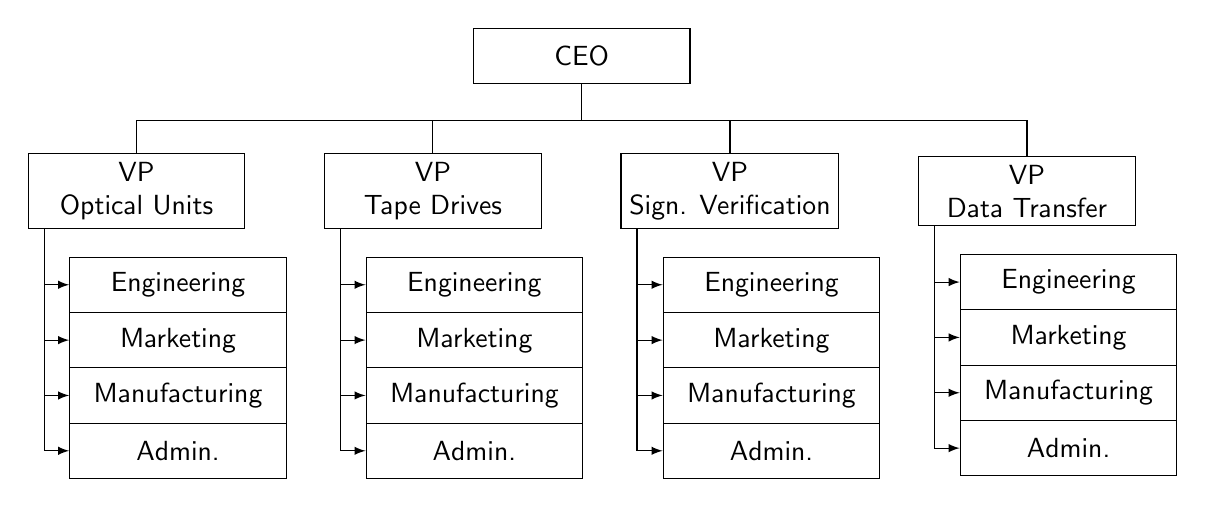
\begin{tikzpicture}[
  level 1/.style={sibling distance=120mm},
  edge from parent/.style={->,draw},
  >=latex,
  every node/.style={basic,inner sep=3pt}
  ]

% The first level
\node[align=center](c1){VP \\ Optical Units};
\node[right= of c1,align=center](c2){VP \\ Tape Drives};
\node[right= of c2,align=center](c3){VP \\ Sign. Verification};
\node[right= of c3,align=center](c4){VP \\ Data Transfer};
\path (c1) -- (c4) node[pos=.5,draw=none](mid){};

% root
\node[above = 1 of mid](root){CEO};

\begin{scope}[node distance=-\pgflinewidth and 1cm]

\node[below = 10pt of c1, xshift=15pt](c11){Engineering};
\node[below =  of c11](c12){Marketing};
\node[below =  of c12](c13){Manufacturing};
\node[below =  of c13](c14){Admin.};

\node[below = 10pt of c2, xshift=15pt](c21){Engineering};
\node[below = of c21](c22){Marketing};
\node[below = of c22](c23){Manufacturing};
\node[below =  of c23](c24){Admin.};

\node[below = 10pt of c3, xshift=15pt](c31){Engineering};
\node[below = of c31](c32){Marketing};
\node[below = of c32](c33){Manufacturing};
\node[below =  of c33](c34){Admin.};

\node[below = 10pt of c4, xshift=15pt](c41){Engineering};
\node[below = of c41](c42){Marketing};
\node[below = of c42](c43){Manufacturing};
\node[below =  of c43](c44){Admin.};

\end{scope}

% lines from root to level 1
\draw (root.south) -- ++(0,-13pt) -| (c1.north);
\draw (root.south) -- ++(0,-13pt) -| (c2.north);
\draw (root.south) -- ++(0,-13pt) -| (c3.north);
\draw (root.south) -- ++(0,-13pt) -| (c4.north);

%coordinate[pos=0.05] (aux) 
% lines from each level 1 node to every one of its "children"
\foreach \value in {1,2,3,4}
  \draw[->] ([xshift=6pt]c1.south west) |- (c1\value.west);

\foreach \value in {1,...,4}
  \draw[->] ([xshift=6pt]c2.south west) |- (c2\value.west);

\foreach \value in {1,...,4}
  \draw[->] ([xshift=6pt]c3.south west) |- (c3\value.west);
  
\foreach \value in {1,...,4}
  \draw[->] ([xshift=6pt]c4.south west) |- (c4\value.west);
  
\end{tikzpicture}


	\end{center}
	
	
	\section*{Problem 7.12}
	\subsection*{\quad(a)}
	For the opening of the new restaurant I suggest the matrix organizational structure as a way to gain ownership of individual projects (in the restaurant business I'd imagine letting things go undone for any length of time means the 	competition beats you out), while maintaining the shared resources of a functional organization. With a new campus restaurant I'd imagine most employees would be wearing more than one hat which could mitigate some of the 		"multi-boss" problems inherent in the matrix structure.
	
	\begin{center}
		
\begin{tikzpicture}[
  level 1/.style={sibling distance=120mm},
  edge from parent/.style={->,draw},
  >=latex',
  every node/.style={basic,inner sep=3pt}
  ]

% The first level
\node[align=center](c1){VP \\ Projects };
\node[right= of c1,align=center](c2){VP \\ Marketing};
\node[right= of c2,align=center](c3){VP \\ Operations};
\node[right= of c3,align=center](c4){VP \\ Purchasing};
\path (c1) -- (c4) node[pos=.5,draw=none](mid){};

% root
\node[above = 1 of mid](root){CEO};

\begin{scope}[node distance=.5cm]

\node[below =  of c1](c11){Research};
\node[below =  of c11](c12){Start Up};
\node[below =  of c12](c13){Opening};
\node[below =  of c13](c14){Operating};

\node[below = of c2](c21){Market Research};
\node[below = of c21](c22){Advertising};
\node[below = of c22](c23){Survey/Feedback};
\node[below = of c23](c24){New Markets};

\node[below = of c3](c31){Site/Menu Research};
\node[below = of c31](c32){Product Design};
\node[below = of c32](c33){Staffing};
\node[below = of c33](c34){Scheduling};

\node[below = of c4](c41){Supply Research};
\node[below = of c41](c42){Init. Purchasing};
\node[below = of c42](c43){Stocking};
\node[below = of c43](c44){Supply};

\end{scope}

% lines from root to level 1
\draw (root.south) -- ++(0,-13pt) -| (c1.north);
\draw (root.south) -- ++(0,-13pt) -| (c2.north);
\draw (root.south) -- ++(0,-13pt) -| (c3.north);
\draw (root.south) -- ++(0,-13pt) -| (c4.north);


%coordinate[pos=0.05] (aux) 
% lines from each level 1 node to every one of its "children"
\def\lastvalue{}
\foreach \value [remember=\value as \lastvalue ] in {1,2,3,4}
  \draw[-] (c1\lastvalue) -- (c1\value.north);

\def\lastvalue{1}
\foreach \value [remember=\value as \lastvalue ] in {2,3,4}
	\draw[dashed] (c\lastvalue1.east) -- (c\value1.west);

\def\lastvalue{}
\foreach \value [remember=\value as \lastvalue ] in {1,...,4}
  \draw[dashed] (c2\lastvalue) -- (c2\value.north);

\def\lastvalue{1}
\foreach \value [remember=\value as \lastvalue ] in {2,3,4}
	\draw[dashed] (c\lastvalue2.east) -- (c\value2.west);

\def\lastvalue{}
\foreach \value [remember=\value as \lastvalue ] in {1,...,4}
  \draw[dashed] (c3\lastvalue) -- (c3\value.north);
  
\def\lastvalue{1}
\foreach \value [remember=\value as \lastvalue ] in {2,3,4}
	\draw[dashed] (c\lastvalue3.east) -- (c\value3.west);
  
\def\lastvalue{}
\foreach \value [remember=\value as \lastvalue ] in {1,...,4}
  \draw[dashed] (c4\lastvalue) -- (c4\value.north);
  
\def\lastvalue{1}
\foreach \value [remember=\value as \lastvalue ] in {2,3,4}
	\draw[dashed] (c\lastvalue4.east) -- (c\value4.west);
  
\end{tikzpicture}


	\end{center}
	
	\subsection*{\quad(b)}
	\subsubsection*{WP\#1}
		\textbf{WP}: Initial Market Survey\newline
		\textbf{Assigned}: Market Research\newline
		\textbf{Objective}: We need to specify the type of restaurant we will be opening. Create and conduct a survey of our market of sufficient size the asks for the type of food the survey would most like to see on campus.\newline
		\textbf{Deliverable}: Raw market research data in a programatically digestible format (preferable JSON or XML).\newline
		\textbf{Method Suggestions}: This may be easier if the survey is conducted through electronic means, but also try to get responses from on-the-ground students. The internet can help a restaurant get exposure, but people 			have to show up or at least actually order food for us to make money. Put boots on the ground.\newline
	\subsubsection*{WP\#2}
		\textbf{WP}: Design Menu\newline
		\textbf{Assigned}: Product Design\newline
		\textbf{Objective}: We need to specify the menu we will be serving. Create a new menu, making sure that what we are serving is based both on the results gained from the Research Project.\newline
		\textbf{Deliverable}: A menu that is clear and consistent with our research.\newline
		\textbf{Method Suggestions}: Make sure that the contents are derived from our research, but take artistic liberty with the look. Understand that the look will have to translate well in both physical and electronic media.\newline
	\subsubsection*{WP\#3}
		\textbf{WP}: Stock Kitchen\newline
		\textbf{Assigned}: Stocking\newline
		\textbf{Objective}: We need to obtain the appropriate food-stuffs and packaging materials.\newline
		\textbf{Deliverable}: A fully stocked kitchen ready for staff to provide all expected orders on Opening Day within reasonable target times meeting quality guidelines.\newline
		\textbf{Method Suggestions}: We know what we are cooking and how. But try to forward-project into problems. If we are quality oriented, will there be a learning curve on any of our dishes? Will that mean wasted product? We 		need the Opening to be a good first impression more than we need it to make money. Purchase accordingly.\newline

	\subsection*{\quad(c)}
	\subsubsection*{WP\#1}
	The Initial Market Survey will need input from the Site/Menu and the Supply Research organizations in order to produce a survey that will lead to actionable intelligence. For instance, if the survey includes questions about alcohol 	availability, but the Site/Menu Research team has discovered that the university does not allow alcohol on campus, then all responses to that question will be mostly moot (it could still give insight into our customer-base, but there 	may be more pertinent question that we could be asking. Customer attention is not an unlimited resource).
	\newline
	In fact, all three teams in the Research project, while have a certain level of autonomy and with their own deliverables, would help the organization at the highest level by keeping the coordination level hight. This should be helped 	by the matrix organization structure. Our projects are aligned temporally, but there will be feedback between the projects until the Opening project is complete and the Operating project is under full swing. Research will have to be 	ready to re-assess if called upon to do so be Opening or Operating project members.
	\subsubsection*{WP\#2}
	The Design Menu package will need a high level of coordination between the Start Up Project and the Research project in order to produce the desired deliverable. The knowledge gain from all three functional groups in the 		Research Project will feed into the decision making processes that takes place during this package. Clarification on survey results and analysis will inform the Start Up Project heavily; conflicting research deliverables will require 		that the Start Up Project and the Research Project are kept in each other's workflow until the Opening Project is complete, at which point the Start Up project resources will be spun into other projects (either new or existing), while 	the Research Project will probably 	continue for some time.
	\subsubsection*{WP\#3}
	The Stock Kitchen package will see the Start Up project's Purchasing resource interacting with the Stocking resource to ensure both amply space and required storage types (if code requirements that come out of the Research 		Project require meats be kept within a certain temperature range, we need to have that equipment). Stock Kitchen will also have to be interacting with Staffing to make sure that the proper amount of product is acquired to both meet 	demand from customers and the training that Staffing will certainly be coordinating. 
	\newline
	There is a high likelihood that the Operating Project will lean heavily on this package for knowledge in how to carry out the day-to-day functions of keeping the restaurant open and generating revenue.
		
	\subsection*{\quad(d)}
	%{\renewcommand{\arraystretch}{1.2} 
	\begin{table}[h!]
  		\begin{center}
    		\caption{LRC for the new restaurant initial survey}
    		\label{tab:table1}
			
    		\begin{tabular}{lcccc}
				Activity & Project & Marketing & Operations & Purchasing\\
				\hline
      			Design Survey & P,R & A,I & I & I\\
      			Administer Survey & R & P &  & \\
				Collect Data & P & R & R & R \\
				Analyze Data & I,A & P & R & \\
				\hline
				
				\multicolumn{5}{c}{Key: I-$>$Informs; A-$>$Approves; R-$>$Reviews; P-$>$Primary} \\
    		\end{tabular}
  		\end{center}
	\end{table}
	%}
	
	\section*{Problem 7.13}
	You have a WBS for opening a new Restaurant on a University Campus
	\subsection*{\quad(a)}
	Develop another WBS and assign the original WPs to nodes in your new WBS.
\end{document}